\documentclass{standalone}
\usepackage{tikz}
\usetikzlibrary{positioning, arrows.meta}

\tikzset{
    block/.style={draw, fill=blue!20, rectangle, 
                  minimum height=3em, minimum width=6em},
    cloud/.style={draw, ellipse,fill=red!20, node distance=3cm,
                  minimum height=2em},
    line/.style={-Stealth, draw},
    cloud/.style={draw, ellipse,fill=red!20, node distance=3cm,
                  minimum height=2em},
    label/.style={draw, fill=yellow!10, rectangle, 
                  minimum height=1.5em, minimum width=8em}
}

\begin{document}

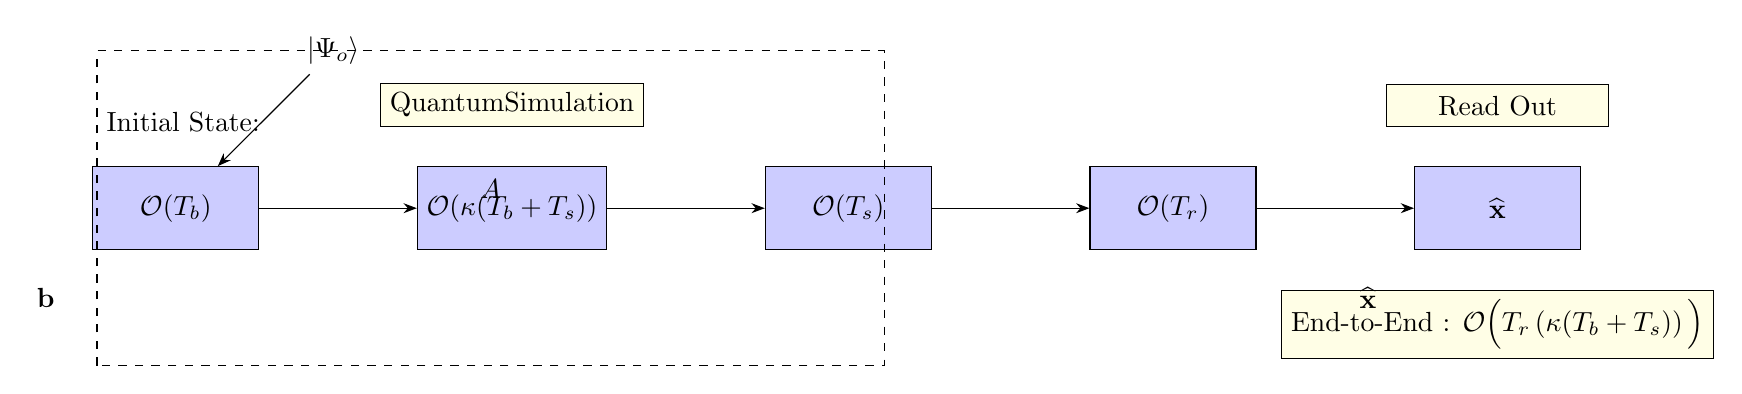
\begin{tikzpicture}[node distance = 2cm, auto]
    % State Initial State
    \node (initial_state) at (0,4) {$|\Psi_o\rangle$};
    \node[below left=0.5cm of initial_state] (initial_label) {Initial State:};

    % Boxes
    \node[block] (op_t_b) at (-2,2) {$\mathcal{O}(T_b)$};
    \node[block] (hhl) [right=of op_t_b] {$\mathcal{O}(\kappa(T_b+T_s))$};
    \node[block] (op_t_s) [right=of hhl] {$\mathcal{O}(T_s)$};
    \node[block] (op_t_r) [right=of op_t_s] {$\mathcal{O}(T_r)$};
    \node[block] (read_out) [right=of op_t_r] {$\widehat{{\mathbf{x}}}$};

    % Quantum Simulation Label
    \node[label] (label_qsim) [above=0.5cm of hhl] {Quantum \\ Simulation};
    \node[label] (label_readout) [above=0.5cm of read_out] {Read Out};
    
    % Read Out Label
    \node[label] (label_final) [below=0.5cm of read_out] {End-to-End : $\mathcal{O}\Big(T_r \left(\kappa (T_b+T_s)\right)\Big)$};
    
    % Arrows
    \path [line] (initial_state) -- (op_t_b);
    \path [line] (op_t_b) -- node[above] {} (hhl);
    \path [line] (hhl) -- node[above] {} (op_t_s);
    \path [line] (op_t_s) -- node[above] {} (op_t_r);
    \path [line] (op_t_r) -- node[above] {} (read_out);
    
    % State Labels
    \node[below left=0.5cm of op_t_b] (state_label) {\textbf{b}};
    \node[below left=0.5cm of read_out] (state_label) {\textbf{$\widehat{{\mathbf{x}}}$}};
    
    % Dashed Box
    \draw[dashed] (-3,0) rectangle (7,4) node[midway, above] {$A$};
\end{tikzpicture}

\end{document}